\documentclass{article}
\usepackage[utf8]{inputenc}
\usepackage{biblatex}
\addbibresource{bibliography.bib}
\usepackage{graphicx}
\usepackage{subcaption}
\usepackage{caption}
\usepackage{siunitx}
\usepackage{hyperref}
\graphicspath{{./images/}}

\usepackage[a4paper, total={6.5in, 8in}]{geometry}

\bibliography{bibliography}

\newcommand*{\ts}{{\tau^{*}}}
\newcommand*{\diff}{\mathop{}\!\mathrm{d}}
\newcommand{\ps}{\si{\pico\second}}
\newcommand{\ns}{\si{\nano\second}}
\newcommand{\ips}{\si{\per\pico\second}}
\newcommand{\us}{\si{\micro\second}} 
\newcommand{\K}{\si{\kelvin}} 

\title{The application of the generalised Langevin equation to surface diffusion and the effect of noise correlations on low-friction activated diffusion processes.}

\author{Jeremy Wilkinson}
\date{September 2021}

\begin{document}

\maketitle

\begin{abstract}
    mucho cool langevin
\end{abstract}

\tableofcontents

\section{Introduction}

Understanding the motion of adsorbed particles over the surface of a substrate is of interest to many fields. Experimental techniques such as helium spin echo microscopy provide insight into adsorbate motion of real systems over a wide range of time and length scales. However, the current experimentally observable quantities, such as the intermediate scattering function, do not provide direct measurements of individual adsorbate trajectories. The interpretation of experimental data therefore requires the introduction of a model for microscopic adsorbate motion to inspire further investigations and technological developments.

At experimentally accessible temperatures, the thermal de Broglie wavelength of most real systems (with the notable exception of Hydrogen adsorbates) are much smaller than typical lattice spacings. This justifies the omission of quantum effects and the use of classical models for such systems. Full molecular dynamics simulations modelling the substrate lattice, adsorbate and their interactions have been used to fit experimental data. This approach has the advantage of capturing the classical phonon-adsorbate interaction entirely. One particular drawback of this approach is the large computational cost associated with simulating the pairwise interactions of thousands of substrate atoms and the adsorbate. 

Langevin dynamics provide an alternative, computationally efficient, approach to modelling inherently chaotic simulations by treating the forces seen by the adsorbate as stochastic and ommiting the substrate from the simulation entirely. The Markovian Langevin equation has been used to succesfully fit the observables of both molecular dynamics and experimental data. However certain anomolous effects such as the temperature dependent friction reported by M Diamant et al suggest there may be discrepencies between molecular dynamics simulations and the Markovian Langevin equation. This paper investigates the effect of removing the Markovian constraint on the stochastic force in the Langevin equation through the use of the generalised Langevin equation and to quantify the effects this has on activated diffusion in the low friction and low temperature regime. 

\section{Langevin dynamics}

The Markovian Langevin equation describes the time evolution of a degree of freedom, such as a particle's position, in the presence of a large chaotic system. Heuristacally speaking, one expects that if a system is sufficiently chaotic then its influence on surrounding particles is, for all intents and purposes, a random variable with equilibrium statistical properties set by the ergodic hypothesis. More concretely, suppose we are interested in the dynamics of a `tagged' particle's position and momentum, $x$ \& $p$, which is interacting with a large collection of particles with position and momentum bundled into the vectors $X$ \& $P$. The force on the tagged particle at any particular instant is purely a function of the particular configuration of $x$ and $X$ with no considerations for the velocities of any particles. The Einstein theory of Brownian motion supposes that over a short time period $\tau$, the \emph{time-averaged} force, $F_n = \int_{n\tau}^{(n+1)\tau}\diff{t'}F(t')$, on the particle of interest is a random variable satisfying the relation $F_n=-m\eta\dot{x}(n\tau) + f_n$ where $\left<f_nf_m\right> = 2k_BTm\eta\delta_{mn}/\tau$. Despite the original system being independent of any velocities, the time averaged force includes a friction term parametrized by a new constant $\eta$ which carries units of inverse time. In this sense, the Langevin equation is a finite difference equation which in the small $\tau$ limit reduces to the well known form $m\ddot{x}(t)=-m\eta\dot{x}(t)+f(t)$ where $\left<f(t_1)f(t_2)\right>=2k_BTm\eta\delta(t_1 - t_2)$. The second condition is reffered to as the fluctuation dissipation theorem and ensures that the particle's kinetic energy satisfies the equipartition theorem, $\left<E_k\right>=\frac{N_d}{2}k_BT$, in $N_d$ spatial dimensions. In Fourier space, this condition is equivelant to $f(t)$ having a uniform power spectral density, $\left<\tilde{f}(\omega_1)\tilde{f}(\omega_2)\right> = (2\pi) 2 k_B T m \eta \delta(\omega_1 + \omega_2)$. This condition is also satisfied by electromagnetic radiation which produces white coloured light and such noise is therefore reffered to as `white'. A term describing the influence of a background potential $U(x)$ may be introduced leading to the equation
\\
\begin{equation}
	\label{eq:markovian_le}
	m\ddot{x}(t)=-m\eta\dot{x}(t) - \nabla U(x(t)) + f(t) \text{ where } \left<f(t_1)f(t_2)\right>=2k_BTm\eta\delta(t_1 - t_2).
\end{equation}
\\
The statistical physics of Equation \ref{eq:markovian_le} is well understood and can be shown to satisfy equilibrium boltzmann statistics, $\rho(x, p)=\frac{1}{Z}\exp(-\beta H(x, p))=\frac{1}{Z}\exp(-\beta(p^2/2m + U(x)))$, exactly for an arbitrary background potential $U(x)$ provided $f$ is a gaussian random variable.

\section{The non-Markovian Langevin equation}

While the Markovian Langevin equation is useful due to its analytic simplicity, the noise in all physical systems is bandlimited and therefore a tagged particle experiences noise correlations in time. One may introduce a memory kernel, $K(t)$, into the Langevin equation to capture these correlations but this modification requires a corresponding change to the friction term to ensure equipartition of energy. This results in the non-Markovian Langevin equation, $m\ddot{x}(t)=-m\eta\int\diff{t'}\dot{x}(t')K(t-t') + \int\diff{t'}f(t')K(t-t')$, which obeys boltzmann statistics exactly in a flat background potential for any memory kernel normalised to have a total area of $1$ (the statistics of $f$ remain unchanged). 

However once a background potential is added to the non-Markovian Langevin equation,
\\
\begin{equation}
	\label{eq:gle}
	m\ddot{x}(t)=-m\eta\dot{x} \star K - \nabla U(x) + f \star K,
\end{equation}
\\
analytical results become sparse and the assumption that the fluctuation dissipation condition is sufficient to ensure equipartition of energy is no longer true. Fortunately it is often a reasonable assumption to make in practice although it is not difficult to construct situations that demonstrate its failure.

\subsection{The exponential memory kernel}

While the form of $K(t)$ is left unconstrained, an exponential memory kernel of the form $K(t)=\theta(t)\frac{1}{\tau}\exp\left(-\frac{t}{\tau}\right)$\footnote{$\theta(t)$ is used here to denote the Heaviside step function.}, parametrized by the correlation time $\tau$, has the advantage of being extremely computationally efficient as one can perform convolutions in linear time. In practice, one can implement such a convolution in a simulation with a timestep of $\Delta{t}$ using
\\
$$
\int_0^{n\Delta{t}} dt' K\left(t-t'\right) \vec{f}(t') \approx \alpha \int_0^{(n-1)\Delta{t}} dt' K\left(t-t'\right) \vec{f}(t') + \frac{1}{1-\alpha} \vec{f}\left(t_n\right)
$$
\\
where the decay factor $\alpha$ is given by $\alpha=\exp(-\frac{\Delta{t}}{\tau})$. The normalisation $\frac{1}{1-\alpha}$ ensures that the total impulse imparted by a force remains unchanged by the discretization process. The power spectrum of $K(t)$ is given by $\left|\tilde{K}(\omega)\right|^2 = \frac{1}{1+\omega^2\tau^2}$ with bandwidth given by the half-width at half-maximum, $w_c=\frac{1}{\tau}$.

While exponential memory kernels are a common choice in the literature, a potentially useful modification which as far as I am aware has not been used before is the exponentially dampened sinusoid, $K(t)=\frac{1+\tau^2\omega_1^2}{\tau}\cos(\omega_1t)\exp\left(-\frac{t}{\tau}\right)$. Such a kernel may be efficiently calculated through a complex decay factor, $\alpha=\exp\left(-\frac{\Delta{t}}{\tau} + i\omega_1\Delta{t}\right)$ and taking the real component of the cumulative force at each timestep. 

The power spectrum of the exponential and dampened sinusoidal kernels are shown in Figure \ref{fig:kernel_spectra}. Together, these functions provide a toolkit for a wide range of kernel spectra, since the exponential kernel may be used as both a high-pass and low-pass filter and the dampened-sinusoid may be used to add or subtract out specific section of the noise spectrum. However when using these exotic kernels in a background potential, one very quickly enters a regime in which the fluctuation-dissipation theorem no longer gaurentees equipartition. 

\begin{figure}
	\centering
	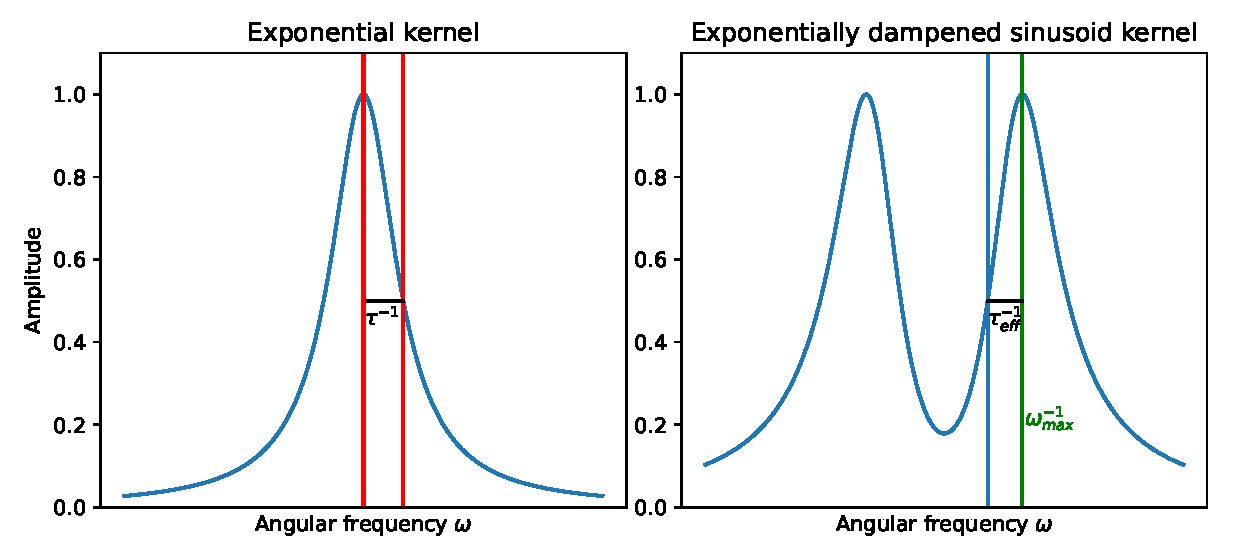
\includegraphics[width=1.0\textwidth]{kernel_spectra}
	\caption{The power spectrum of the exponential and exponentially dampened sinusoidal kernel. The exponential kernel is centered around $0$ with a half-width at half-maximum of $\tau^{-1}$. The exponentially dampened sinusoidal kernel is centered at $\omega_{\text{max}} \approx \omega_1$ with a half-width at half-maximum of $\tau_{\text{eff}}^{-1}\approx\tau^{-1}$.} 
	\label{fig:kernel_spectra}
\end{figure}


\section{Models for activated diffusion in the low-friction regime}

Models for the escape of a particle over a potential barrier, known as the Kramers problem, have been studied for many decades. Many such models are built within the framework of the Markovian Langevin equation in the presence of a background potential. The background potential is assumed to contain an approximately harmonic potential trap of barrier height $E_a$ which the particle is able to escape to a region from which the particle never returns, as in Figure \ref{fig:kramers_potential}. 

The qualative behaviour of the particle's dynamics varies significantly across parameter ranges. For the purposes of this paper, we restrict the discussion to the low friction regime, that is to say, diffusion in a system for which $\frac{\eta}{\omega_0} << 1$ where $\omega_0$ is the natural angular frequency of the trapping well. The defining feature of this regime is that the particle changes its total energy very slowly and so the particle is able to oscillate many times without its total energy changing significantly. Furthermore if the particle does find itself at the top of the potential well, the likelihood of the particle diffusing around the potential maximum, changing directions repeatedly and making so called `multiple crossings' of the barrier, is small. Using these assumptions, one may derive expressions for the escape rate of a particle over the barrier of an Ahrennius form, 
\\
$$\gamma = A \eta \exp\left(-\beta E_a \right).$$ 
\\
The factor $\eta A$ is reffered to as the pre-exponential factor of the hopping rate and while in principal $A$ is temperature dependent, in practice, $A$ is often treated as temperature independent as most of the temperature dependence is found in exponential factor (really?). The key theoretical result for our purposes is that the pre-exponential factor is found to be proportional to the friction constant $\eta$ for low-friction systems.

While not a rigorous exercise, it is helpful to loosely interpret the features in the Ahrennius equation. We consider a statistical model for escape over the barrier in which the particle is consistently, but slowly, changing its energy with a typical energy correlation time reffered to as the \emph{time to forget}, $\phi$. In the Markovian Langevin equation $\phi$ is equal to $\eta^{-1}$ as the energy auto-correlation function $\left<E(0)E(t)\right>$ decays exponentially with a decay rate given by $\eta$.  The number of independent energy levels which the particle achieves per unit time is given by $\phi^{-1}$ and each time the particle achieves an energy level greater than the barrier height, we assume the particle has some probability of escaping the well before its energy changes to some new independent value. In a one dimensionsal system, this probability is close to unity, however things are more complicated for higher dimensional systems in which the activation site isn't rotationally symmetric and the particle can explore the well at energies higher than the activation energy without actually finding the bridge point. We further assume that the probability of escape given sufficient energy is insensitive to small variations in $\phi$. Within this statistical framework, the Ahrennius equation can be loosely interpreted as the product of the rate at which the particle changes its energy, $\phi^{-1}$, the probability that the particle changes its energy to a value greater than the barrier energy, $\exp(-\beta E_a)$, and the probability of escape given an energy level greater then $E_a$, $A$. 

\begin{figure}
	\centering
	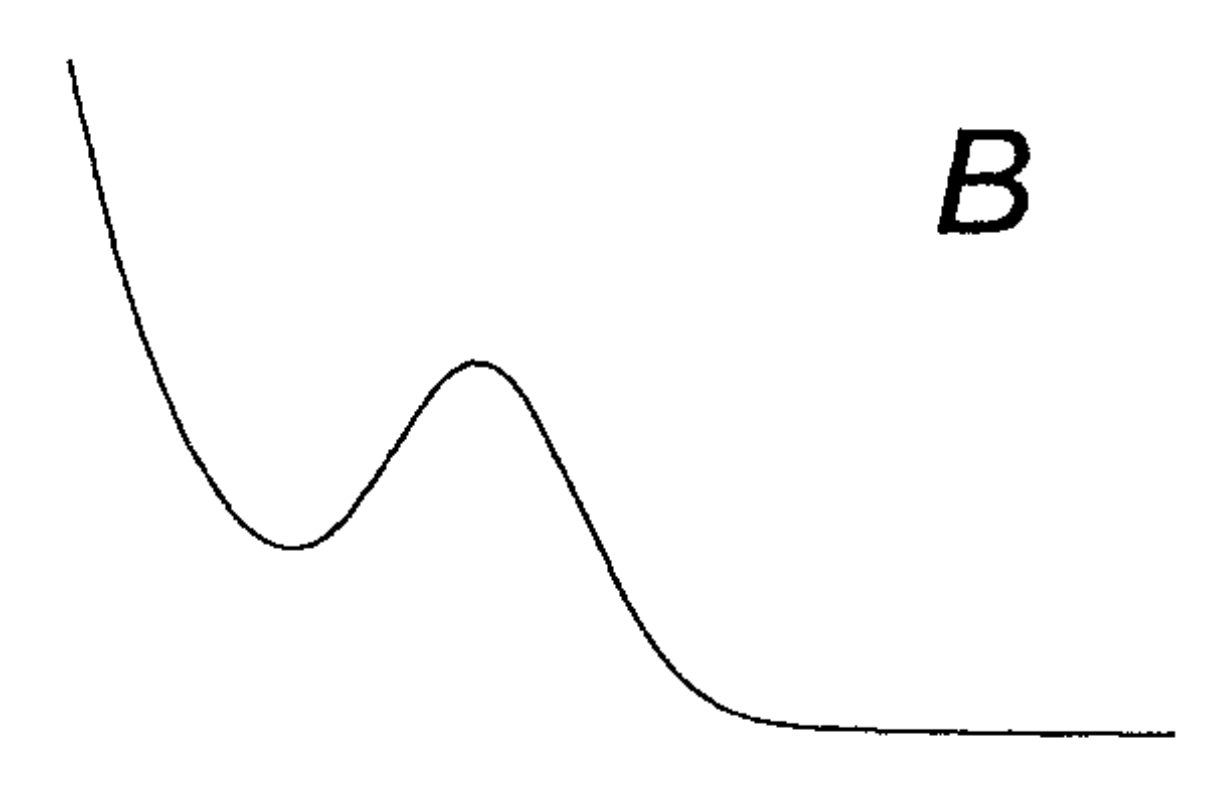
\includegraphics[width=0.6\textwidth]{kramers_potential}
	\caption{}
	\label{fig:kramers_potential}
\end{figure}

\section{Basic definitions and methods for spectra interpretation}

\section{Hopping rates and the effect of high frequency phonons}

The Markovian Langevin equation implicitly assumes that the correlation time of the Langevin noise term is infinitesimally small, that is to say, $\left< f(t_1) f(t_2) \right> = \sigma^2 \delta (t_1 - t_2)$. In Fourier space, this condition is equivelant to the statement that the power spectrum of the noise is uniform, $\left< \tilde{f}(\omega_1) \tilde{f}(\omega_2) \right> = 2 \pi \sigma^2 \delta(\omega_1 + \omega_2)$. However all real systems are bandlimited and in the case of surface dynamics the noise cutoff manifests as the phonon cutoff frequency of the substrate. Even in an idealised Langevin simulation, the spectrum of the simulated noise cannot excede $\frac{1}{2\delta{t}}$, where $\delta{t}$ is the timestep of the simulation, and so the effects of ommitting high frequency noise components need to be understood to be safely neglected. 

If no background potential is present, the solution to the Langevin equation may be expressed as a simple integral over a Green's function, $F(t)$, satisfying $\ddot{F} + \eta \dot{F} = \delta(t)$,

$$
x(t) = \frac{1}{m} \int_{-\infty}^t \diff{t'} f(t') F(t-t') \longrightarrow \tilde{x}(\omega) = \frac{1}{m} \tilde{f} \tilde{F}.
$$ 

In this case the removal of high frequency noise components in $\tilde{f}$ simply amounts to the removal of these same noise components from the trajectory of the particle. From this analysis it may be expected that high frequency noise components only affect the short time-scale motion of the particle but leave the macroscopic trajectory unchanged, as demonstrated in Figure \ref{fig:noise_trajectories}. However in the presence of an anharmonic background potential, the Langevin equation ceases to be linear in $x$ and the compounding of small differences between trajectories causes macroscopic divergence between trajectories which otherwise only differ in high frequency noise components. While this does not immediately imply that statistical properties taken over an ensemble of trajectories will be affected, one cannot assume that long-time scale observables are unaffected by high frequency noise in the non-linear case.

\begin{figure}
	\centering
	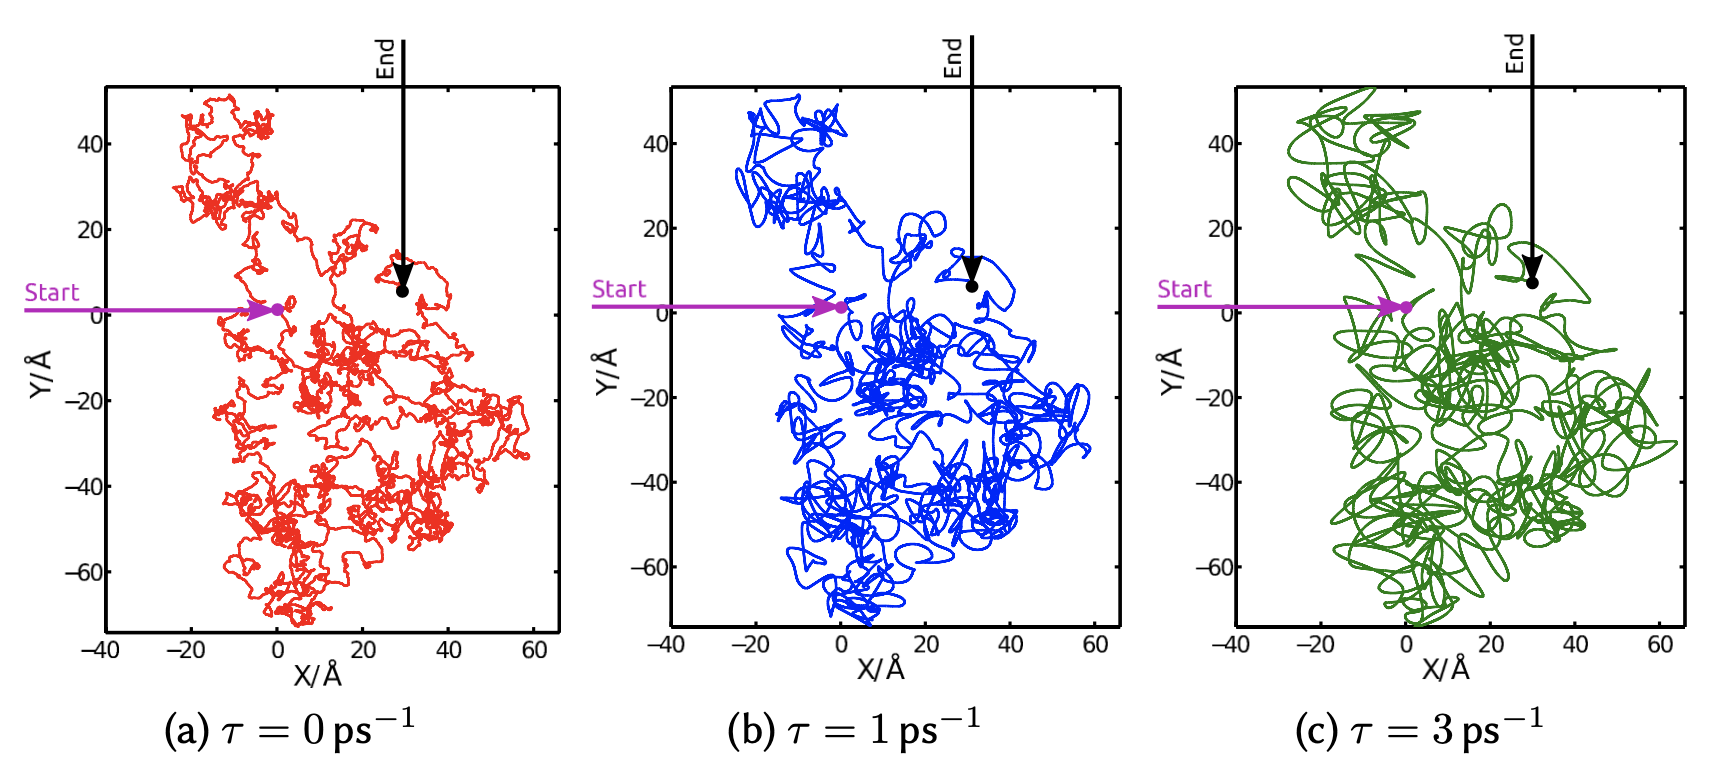
\includegraphics[width=0.8\textwidth]{noise_trajectories}
	\caption{A demonstration of how the introduction of bandlimited noise affects the trajectory of a particle.}
	\label{fig:noise_trajectories}
\end{figure}

\subsection{Evaluation of the effect of high frequency noise on the hopping rate of Sodium on Copper(001)} \label{sec:hopping_simulations}

A Langevin simulation was constructed using a potential energy surface extracted from a molecular dynamics model of Sodium adsorbed on Copper(001) as presented in \cite{Gil}. An exponential memory kernel of the form $K(t) = \frac{1}{\tau}\exp(-t/\tau)$ was introduced to control the bandwidth of the noise. The noise correlation time $\tau$ is related to the bandwidth of the noise through the relation $\tau = \frac{1}{2 \pi f_c}$ where $f_c$ is the frequency at which the power spectrum of the noise is reduced to half its peak value. 

A GLE simulation was run for $2\us$ for each value of $\eta\in\left[0.4, 0.8\right)\ips$ and $\tau\in\left[0, 0.4\right)\ps$ in steps of $0.01$ at a temperature of $300\K$. The simulated trajectories were used to calculate the long-time decay rate of the ISF as well as the decay rate of the total energy auto-correlation function. The results of these simulations are summarized in Figure \ref{fig:ttf_gamma}.

Figure \ref{fig:gamma_and_ttf_contours} demonstrates the non-trivial dependence of the system's time to forget and ISF decay rate on $\eta$ and $\tau$. From these results it is evident that correlations in the system's noise can have a strong effect on the hopping rate of the adsorbate. Although the ISF decay rate is a function of both $\eta$ and $\tau$, the alignment of the contours of $\phi^{-1}$ and $\Gamma$ shows that, for a given temperature and background potential, $\Gamma$ is parametrized by only one parameter, the systems time to forget, and is independent of the orthogonal parameter.

The relationship between $\Gamma$ and $\phi$ is shown in Figure $\ref{fig:gamma_and_ttf_scatter}$ and is observed to be linear in $\phi^{-1}$ apart from the $\phi^{-1} \rightarrow 0$ limit. This departure from linearity may be attributed to the probability of hopping being affected by the time to forget in this limit.  

\begin{figure}
	\centering
	\begin{subfigure}{1.0\textwidth}
		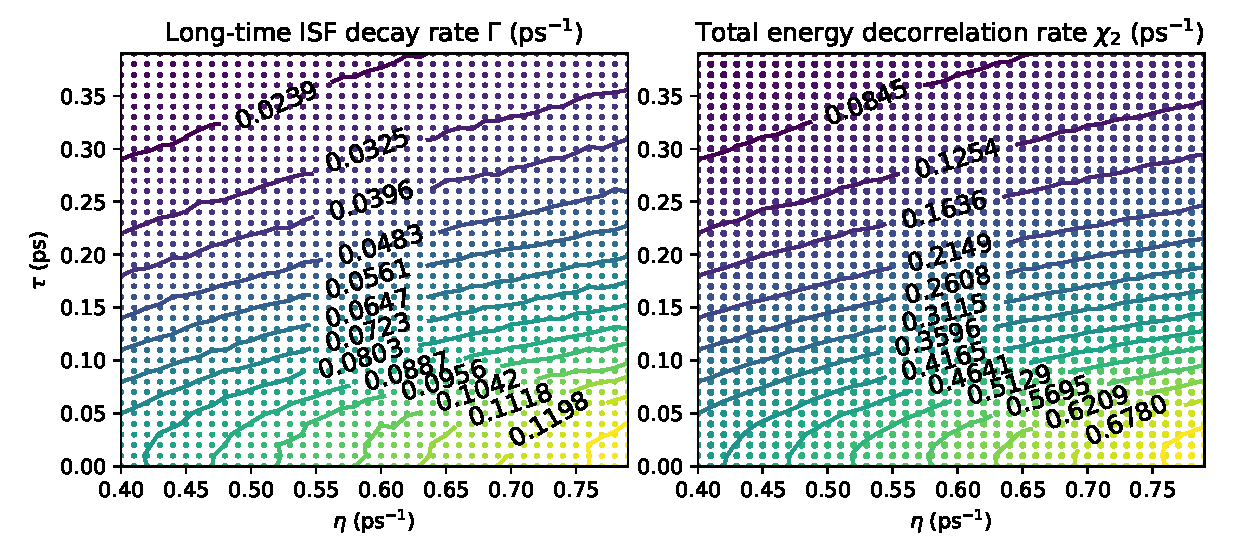
\includegraphics[width=1.0\textwidth]{gamma_and_ttf_contours}
		\caption{Contour plots of the long-time ISF decay rate, $\Gamma$, and the decay rate of the total energy auto-correlation function, $\chi_2$ as functions of $\eta$ and $\tau$. The alignment of the contours implies that, in this parameter regime, the pre-exponential factor of the hopping rate is solely a function of the system's `time to forget'.}
		\label{fig:gamma_and_ttf_contours}
	\end{subfigure}
	\begin{subfigure}{1.0\textwidth}
		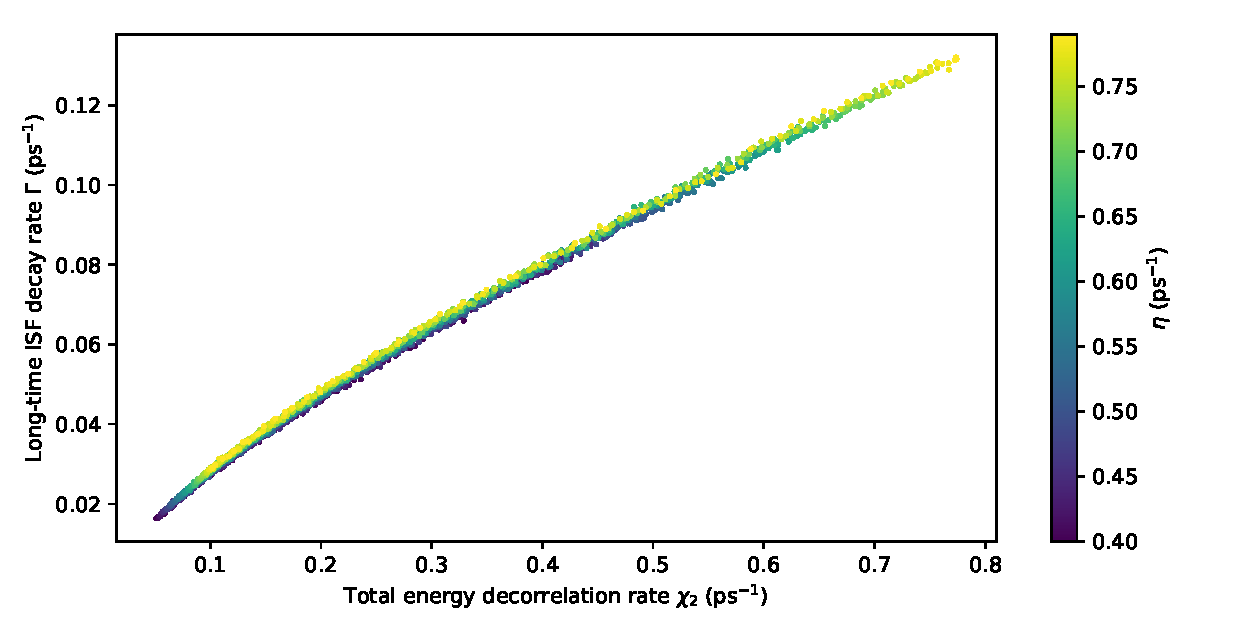
\includegraphics[width=1.0\textwidth]{gamma_and_ttf_scatter}
		\caption{The relationship between the kinetic energy decay rate and the ISF decay rate is observed to be linear except in the small $\chi_2$ limit. The colour of each marker is set by the value of $\eta$ for the simulation and further demonstrates that $\Gamma$ is not solely function of $\eta$.}
		\label{fig:gamma_and_ttf_scatter}
	\end{subfigure}
	\caption{}
	\label{fig:ttf_gamma}
\end{figure}

\subsection{Theoretical models of a system's time to forget} 

The time to forget of a system can be better understood through the study of some simple theoretical models. The simplest case of a particle with Langevin statistics in a flat potential has a time to forget of $\phi=\frac{1}{2\eta}$ whereas the introduction of a harmonic background potential, $V(x)=\frac{1}{2}m\omega_0^2x^2$, results in a longer time to forget of $\phi=\eta^{-1}$. This difference can be traced back to the fact that the energy of the particle in a harmonic well spends half its time in potential form where it remains unaffected by friction. If a noise cutoff is introduced to the harmonic system in the form of the aforementioned exponential memory kernel, things complicate considerably and the time to forget becomes a non-trivial function of $\eta$, $\tau$ and $\omega_0$. The functional form of these relationships depend on the exact pole structure of the Green's function of the system and its qualitive behaviour can vary drastically in a similar fashion to an under vs overdamped oscillator.

As a model for the corrugated periodic potential of a substrate, Figure \ref{fig:compare_theoretical_ttf} compares the time to forget of the corrugated potential to the time to forget of an equivalent harmonic well with the same curvature as the potential minimum of the corrugated potential of Section \ref{sec:hopping_simulations}. The results indicate that the time to forget of the harmonic well is only a reasonable approximation for low levels of $\tau$ with the error rapidly reaching 40\%. This is attributed to deviations of the corrugated potential from the harmonic potential becoming pronounced around the typical thermal energies at $300\K$. To be run again at lower temperatures. 

\begin{figure}
	\centering
	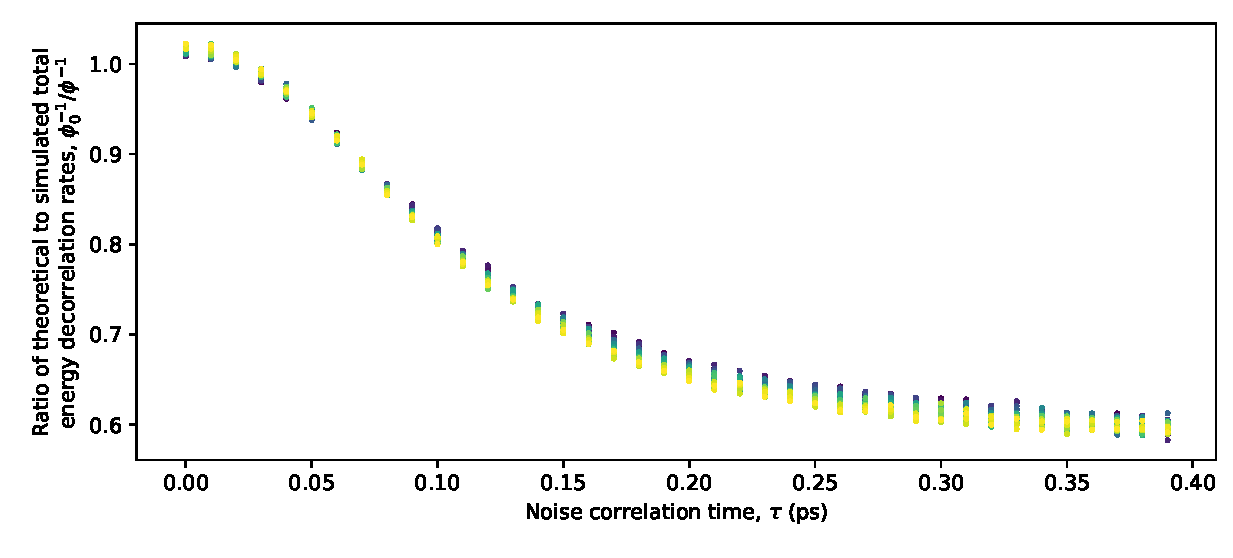
\includegraphics[width=1.0\textwidth]{theoretical_ttf_comparison}
	\caption{}
	\label{fig:compare_theoretical_ttf}
\end{figure}

\section{Temperature dependent friction and the effect of low frequency phonons}

While the upper bound of the phonon noise spectrum is set by the inter-atomic spacing of the lattice, the lower bound is set by the size of the substrate. The length of the substrate fixes a maximum phonon wavelength with a corresponding minimum vibrational frequency. While physical substrates are well approximated by an unbounded system, 3D molecular dynamics simulations are severly limited in system size due to computational cost. The paper by \ref{Gil} explores the ability of a Langevin simulation to fit a full 3D model of Na on Cu(001). This paper found that the friction parameter required to fit the observed data increased as a function of temperature. The 3D simulations in the aforementioned paper were performed with a crystal of size $8\times8\times8$ which suggests that these effects may be an artefect of finite system size. To test this hypothesis, the simulation setup was recreated across three separate system sizes, $8^3$, $16^3$ and $32^3$. Each system was randomly initialized and allowed to run for $10\ns$ for $200$ iterations with a cumulative runtime of $2\us$. It is important to re-initialize the substrate accross iterations so substrate energy can be shuffled between stable phonon modes. From each simulation, the ISF dephasing rate as a function of momentum transfer was calculated in the same fashion as described  

\begin{figure}
	\begin{subfigure}{1.0\textwidth}
		\centering
		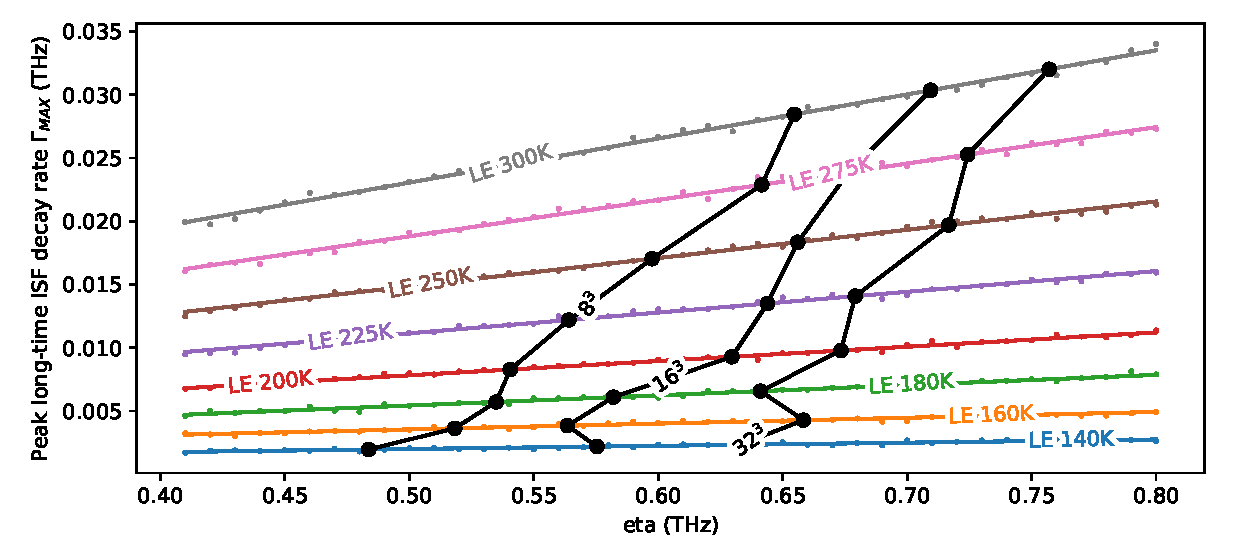
\includegraphics[width=1.0\textwidth]{md_vs_gle_gamma}
		\caption{}
		\label{fig:md_vs_gle_gamma}
	\end{subfigure}
	
	\begin{subfigure}{1.0\textwidth}
		\centering
		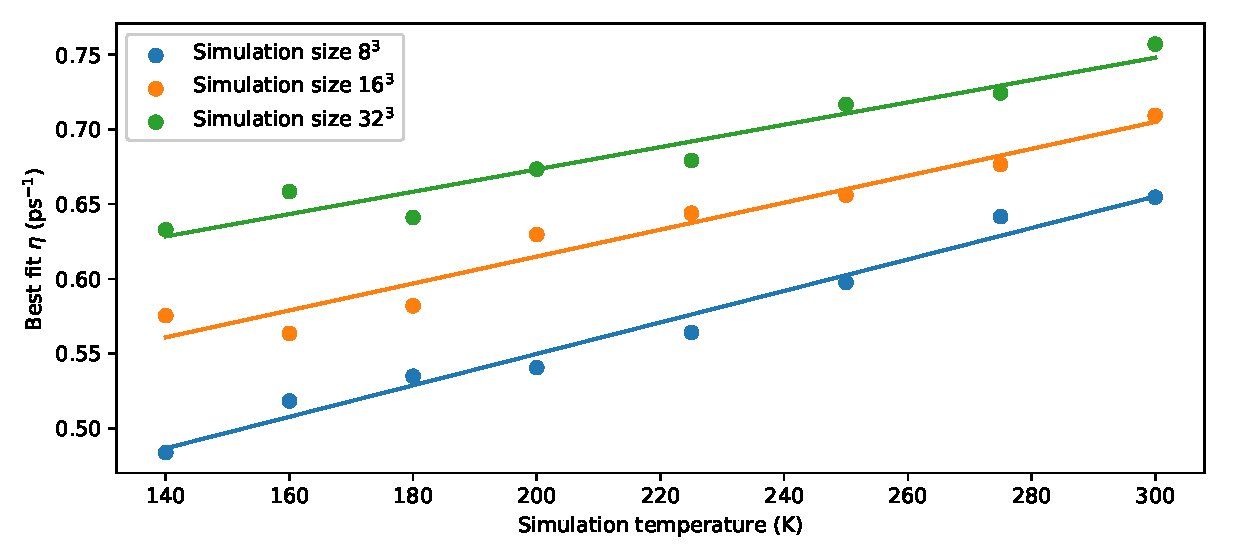
\includegraphics[width=1.0\textwidth]{md_temp_vs_eta}
		\caption{}
		\label{fig:md_temp_vs_eta}
	\end{subfigure}
\end{figure}

The potential energy surface isn't changed

\section{Summary}

$w_0=48$

test

\end{document}
